\documentclass{standalone}

\usepackage{pgfplots}
\usepgfplotslibrary{polar}
\pgfplotsset{compat=1.10}

\pgfplotsset{mypolarplot/.style={%
  clip=false, % needed for double line (last \addplot command)
  domain=0:360, % plot full cycle
  samples=180, % number of samples; can be locally adjusted
  grid=both, % display major and minor grids
  major grid style={black}, 
  minor x tick num=3, % 3 minor x ticks between majors
  minor y tick num=1, % 1 minor y tick between majors
  xtick={0,45,...,359},
  xticklabels={%
    $0$,
    $\frac{ \pi}{4}$,
    $\frac{ \pi}{2}$,
    $\frac{3\pi}{4}$,
    $\pi$,
    $\frac{5\pi}{4}$,
    $\frac{3\pi}{2}$,
    $\frac{7\pi}{4}$
  },
  yticklabel style={anchor=north}, % move label position
}}

\begin{document}
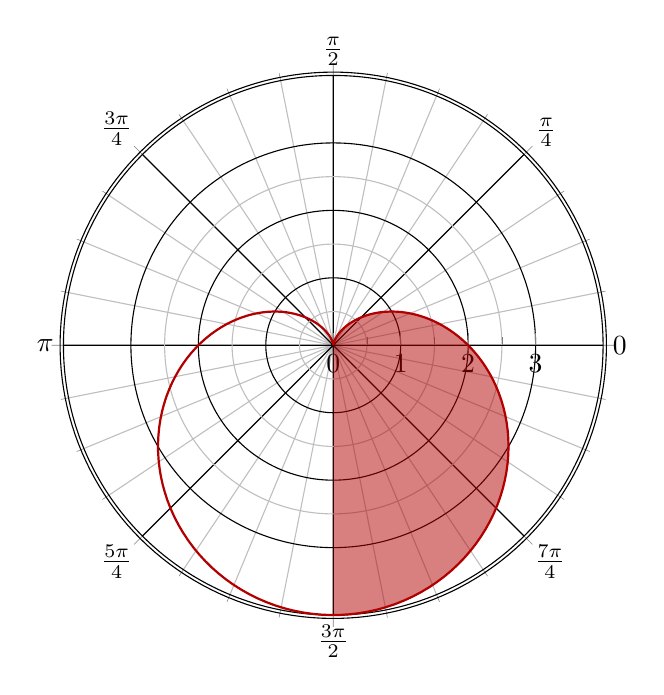
\begin{tikzpicture}
\begin{polaraxis}[%
  ymax=4,
  ytick={0,1,2,3},
  mypolarplot,
]
  \addplot[mark=none,fill=red!70!black,opacity=0.5,domain=-90:90] {2-2*sin(\x)};
  \addplot[mark=none,thick,red!70!black] {2-2*sin(\x)};
  \addplot[black] {4.05}; % there is likely a better way to do this
\end{polaraxis}
\end{tikzpicture}
\end{document}